%
% File acl2018.tex
%
%% Based on the style files for ACL-2017, with some changes, which were, in turn,
%% Based on the style files for ACL-2015, with some improvements
%%  taken from the NAACL-2016 style
%% Based on the style files for ACL-2014, which were, in turn,
%% based on ACL-2013, ACL-2012, ACL-2011, ACL-2010, ACL-IJCNLP-2009,
%% EACL-2009, IJCNLP-2008...
%% Based on the style files for EACL 2006 by 
%%e.agirre@ehu.es or Sergi.Balari@uab.es
%% and that of ACL 08 by Joakim Nivre and Noah Smith

\documentclass[11pt,a4paper]{article}
\usepackage[hyperref]{acl2018}
\usepackage{times}
\usepackage{latexsym}
\usepackage{amsmath}
\usepackage{amssymb}

\usepackage{graphicx}
\graphicspath{ {pictures/} }

\usepackage{url}

\aclfinalcopy % Uncomment this line for the final submission
%\def\aclpaperid{***} %  Enter the acl Paper ID here

%\setlength\titlebox{5cm}
% You can expand the titlebox if you need extra space
% to show all the authors. Please do not make the titlebox
% smaller than 5cm (the original size); we will check this
% in the camera-ready version and ask you to change it back.

\newcommand\BibTeX{B{\sc ib}\TeX}

\title{ANLP and IR project - Attentive pooling in \textit{CNN} and \textit{biLSTM} - A word-embedding comparison}

\author{Martina Paganin and Luca Di Liello \\
  Universit\`a degli studi di Trento \\
  {\tt martina.paganin@studenti.unitn.it
       luca.diliello@studenti.unitn.it} \\
}

\date{16/10/2018}

\begin{document}
\maketitle
\begin{abstract}
In the field of Natural Language Processing and Information Retrieval, the task of question answering/answer selection is one of the most important.
In this context, Attentive Pooling networks have been proposed. Based on a previous work, two alternative networks have been implemented: \textit{CNN} and \textit{biLSTM}. Both the networks have a final common step consisting in the Attentive Pooling phase.
This work has been re-proposed with different embedding models, in order to study its behavior under different implementations.
Finally, several tests have been performed on two different datasets, to find a good combination of network parameters and to find the best embedding model.

\end{abstract}

\section{Introduction}

This paper reports the development of a method proposed in Attentive Pooling Networks, by Dos Santos et al\cite{mainpaper}. This methodology aims at building a model, more specifically, a neural network, which has to learn how to recognise correctness of answers given a question.

Attentive Pooling has to learn a similarity measure over pairs of question-answer in order to perform the ranking. 

According to the aforementioned paper, the attentive pooling step improves traditional neural network (\textit{CNN} and \textit{biLSTM}) performances. 
Our implementation reproduces the method proposed in the paper, with some slight differences to explore how different embedding models can affect the already existing implementation. These will be discussed in the following sections.

\section{Methodology}
The method proposed reflects the structure suggested by the referenced paper, so both a \textit{CNN} and a \textit{biLSTM} were implemented following the scheme and the instructions explained in the paper.

Detailed explanations of the two networks and the attentive pooling method follow in the next subsections.

Both networks work on inputs in an embedded form. This means that, first of all, fixed-length independent continuous vector representations are computed. Then, the networks proceed through different steps.

Finally, both methods operate max-pooling and then compute cosine similarity between question and answers representations. 

\subsection{The \textit{CNN}}

The paper suggests to create a particular input representation (called $Z$ vector) before the convolution phase. This vector holds information for each word, such as previous and following words in the sequence. Given a neighbourhood of size $k$, a question/answer length $m$ and an embedding size $d$, the $Z$ vector has a size of $kd$ x $m$ and each column $i$ contains $k$ embedded words centralized on the $i$-th word of the original sentence. Follows an example with $k$ equal to $3$.
\[
\begin{bmatrix}
    w_0 & w_1 & \dots & w_m \\
\end{bmatrix}
 \rightarrow
\begin{bmatrix}
    0 & w_0 & \dots & w_{m-1} \\
    w_0 & w_1 & \dots & w_m \\
    w_1 & w_2 & \dots & 0 \\
\end{bmatrix}
\]

\begin{table*}[h]
  \centering
  \begin{tabular}{|l|c|c|c|c|c|}
    \hline
    \bf Part & \bf \# entries & \bf \# pos answers & \bf \# neg answers & \bf question len & \bf answers len \\
    \hline
    Train & 1161 & 5.43 & 40.49 & 7.38 & 24.80 \\
    Validation & 69 & 3.52 & 15.94 & 6.70 & 24.30 \\
    Test & 68 & 3.65 & 17.56 & 7.43 & 21.84 \\
    \hline
  \end{tabular}
  \caption{Average statistics on $TrecQA$ dataset}
  \label{table:statstrec}
\end{table*}

\begin{table*}[h]
  \centering
  \begin{tabular}{|l|c|c|c|c|c|}
    \hline
    \bf Part & \bf \# entries & \bf \# pos answers & \bf \# neg answers & \bf question len & \bf answers len \\
    \hline
    Train & 856 & 1.19 & 8.91 & 6.04 & 21.10 \\
    Validation & 122 & 1.11 & 8.11 & 6.17 & 20.32 \\
    Test & 235 & 1.20 & 8.63 & 6.06 & 20.69 \\
    \hline
  \end{tabular}
  \caption{Average statistics on $WikiQA$ dataset}
  \label{table:statswiki}
\end{table*}

Both question and answer are processed by the same network in order to derive the same weights matrix. The number of convolutional filters is chosen equal to $4000$ as reported in the aforementioned paper but in the version without AP it can also be slightly decreased (to $3600$).

\subsection{The \textit{biLSTM}}
The bidirectional $LSTM$ network takes as input embedded questions and answers, as the previous described convolutional neural network. This kind of network has the ability of processing the sequence in two directions, using both the information about past and future tokens.
This implements a sort of memory mechanism, allowing the network to "remember" the previous inputs and be more suitable to processing sentences.
In our implementation the hidden vector size was chosen as the one suggested in the paper (282).

Running this kind of network takes considerably more time compared to the \textit{CNN} if considering a number of convolutional filters similar to the number of hidden units, due to the fact that the latter has a less complex structure and then a faster training phase. \textit{biLSTM}s have instead to learn and remember more information and their execution is consequently more computational expensive. Moreover each batch requires the generation of new hidden vectors with an appropriate size.

\subsection{Attentive Pooling}

Attentive Pooling is the method proposed by the authors of the referenced paper to improve the discriminative models performance on pair-wise ranking. It consists in building a kind of common map for words, with score values that are independent from the position that a term can occupy inside a question/answer. This layer aims at learning the representations of both inputs and their similarity measurement. The main idea is learning the similarity between the two inputs and then performing a pooling phase on the previously obtained vectors. 
Attentive pooling can be applied to \textit{CNN}s and also to \textit{RNN}s, and in this experiment it can be found as final step in the model.

\begin{table*}[t]
  \centering
  \begin{tabular}{|c|c|c|c|c|c|}
    \hline
    \bf Network structure & \bf context\_window & \bf filters\_number & \bf batch\_size & \bf learning\_rate & \bf loss\_margin \\
    \hline
    \textit{CNN} & 3 & 3600 & 20 & 1.1 & 0.5 \\
    \textit{biLSTM} & 1 & 282 & 20 & 1.1 & 0.1 \\
    \textit{AP-CNN} & 4 & 400 & 20 & 1.1 & 0.5 \\
    \textit{AP-BiLSTM} & 1 & 282 & 15 & 1.1 & 0.2 \\
    \hline
  \end{tabular}
  \caption{Best parameters for each networks structure}
  \label{table:params}
\end{table*}

\begin{table}[h]
    \begin{center}
        \begin{tabular}{|c|c|}
        \hline
        question & pos\_answer \\
        \hline
        question & neg\_answer \\
        \hline
        question & neg\_answer \\
        \hline
        \vdots & \vdots \\
        \hline
        question & neg\_answer \\
        \hline
        \end{tabular}
    \caption{A batch entry}
    \label{table:entry}
    \end{center}
\end{table}

\subsection{Word Embedding model}
As said in the previous sections, the input for the two networks is in an embedded form, so an embedding layer is necessary in the first phase. Embedding models are useful for computing vector representation of words, and to accomplish this task, PyTorch library provides a dedicated neural network module for word embedding. Moreover, word embedding models avoid the giant dimensional space needed by other methods, such as the one-hot encoding.
The PyTorch module allows to encode words as vectors of real numbers, which is an essential processing phase in $NLP$ tasks.
The PyTorch embedding layers allows both the online learning of the word embedding while training the network and the load of a pre-trained models such as the ones developed by Facebook, Google and the Stanford University \cite{w2v} \cite{glove} \cite{wiki}. This models are trained on very large datasets of text such as Wikipedia's dumps or news collections.

In our implementation, we tested 4 different pre-trained models and two different ways of learning the word embedding in an online manner. All the details, description and comparisons follow in section 6.

\section{Datasets description and preparation}

Two different datasets were used to train and test the architectures: the $TrecQA$ (Text REtrival Conference) Question Answer dataset (8-13) \cite{trec} and the $WikiQA$ dataset developed by Microsoft \cite{wikids}.

These datasets are organized as a list of candidate answers for each one of the questions. The answers are tagged as positive or negative according to their correctness with respect to the related question. Tables \ref{table:statstrec} and \ref{table:statswiki} show some statistics about the two datasets.

The networks are trained by feeding them with batches composed of tuples. A batch is composed of different entries, where each one is a list of up to $50$ tuples. Table \ref{table:entry} shows an example of entry. Given that each entry needs at least a question with a negative and a positive answer, the datasets has been filtered to remove questions with only negative or with only positive answers.

\section{Tests for parameters setting}

Several tests were done, on both the two datasets, in order to try different parameter combinations and find the best one for each network structure. Parameters that need to be found are $k$ (the context window), the batch size $bs$, the learning rate $lr$ and the margin loss $ml$. The number of epochs was fixed at $25$. As in the original paper, the best parameter configuration was decided to be the same for both datasets, in order to have a more dataset-independent network, able to better generalize with respect to different contexts.

MRR and MAP were then computed by trying different combination of the parameters listed above. 

For the $TrecQA$ dataset, combinations that tend to maximize both these two indexes are those with batch size equal to $20$ and an initial learning rate equal to $1.1$. The learning rate is then linearly decreased at each epoch. To assure better results on \textit{CNN} architectures it is better to set $k$ to $3$/$4$ as the context window for the convolution phase. 

Moreover, the loss margin used in the hinge loss function should be set to $0.5$ and $0.1$ for the \textit{CNN} and \textit{biLSTM} architectures respectively.

Each entry of a batch is a sequence of up to $50$ tuples allowing the use of a hard negative training technique. However, lot of questions do not have so many negative answers and than there are lot of entries shorter than $50$ tuples.

These parameters were mantained also during the testing phase on the $WikiQA$ dataset. Table \ref{table:params} summarizes the best combination of parameters found for each network architecture.

\section{Results and discussion}

\begin{table}[h]
\begin{center}
\begin{tabular}{|l|l|l|}
\hline \bf Network structure & \bf MAP & \bf MRR \\ 
\hline
\textit{CNN} & 0.70 & 0.79  \\
\textit{biLSTM} & 0.72 & 0.79  \\
\textit{AP-CNN} & 0.66 & 0.77  \\
\textit{AP-BiLSTM} & 0.66 & 0.76 \\
\hline
\end{tabular}
\end{center}
\caption{Results on $TrecQA$}
\label{table:trecres}
\end{table}

\begin{table}[h]
\begin{center}
\begin{tabular}{|l|l|l|}
\hline \bf Network structure & \bf MAP & \bf MRR \\ \hline
\textit{CNN} & 0.66 & 0.66  \\
\textit{BiLSTM} & 0.65 & 0.65  \\
\textit{AP-CNN} & 0.64 & 0.68  \\
\textit{AP-BiLSTM} & 0.63 & 0.67 \\
\hline
\end{tabular}
\end{center}
\caption{Results on $WikiQA$}
\label{table:wikires}
\end{table}

Table \ref{table:trecres} and \ref{table:wikires} report results obtained with the best combination of parameters that was found. As can be seen, results on $WikiQA$ are generally lower for all the $4$ architectures. This may be due to the fact that $WikiQA$ dataset has fewer entries ($856$ vs $1161$) and a bigger test set. Moreover, for each question it has a lower number of positive answers and this may affect the composition of the batch entries.

Analyzing results obtained on $TrecQA$, it can be noticed that the best performing network is \textit{biLSTM}, followed by \textit{CNN}, while versions with AP delivered lower results maybe due to slower convergence related to hardware limitations.

\section{Performances of embedding models}

Now it follows a comparison of different word embedding models, to show how they can affect performances. All the tests have been done on the same machine to make fair time comparisons. 6 different ways of embedding words were taken into account:
\begin{itemize}
    \item $Google$: The GoogleNews word2vec model \cite{w2v}, containing about 3 million words. It is trained on a very large dataset of news, as the name suggests.
    \item{$GoogleRed$: A reduced version of the GoogleNews word2vec model \cite{git}, containing about $300.000$ words, filtered with the help of English dictionaries. }
    \item{$Glove$: The Glove word2vec model developed by the Stanford University \cite{glove}.}
    \item{$Wiki$: word2vec model developed by Facebook-research team \cite{wiki}, trained on Wikipedia and containing abount a 1 million words.}
    \item{$LearnPyTorch$: let the PyTorch embedding layer \cite{embedding} learn the best word embedding while training the Question-Answer network.}
    \item{$LearnGensim$: create a word2vec model using Gensim \cite{gensim} on the datasets before training the Question-Answer network.}
\end{itemize}
All embedding models will create, for each word, fixed size vectors $v \in \mathbb{R}^{300}$

Before explaining the results in performances, a note about the time impact of different models on the training phase (all models are in binary format):
\begin{itemize}
    \item $Google$: $89.6s$ to be loaded.
    \item $GoogleRed$: $9.3s$ to be loaded.
    \item $Glove$: $10.6s$ to be loaded.
    \item $Wiki$: $26.7s$ to be loaded.
    \item $LearnPyTorch$: it does not need to be loaded but gives a $\sim20\%$ increase in training time. \item $LearnGensim$: needs about $93s$ to be trained on TrecQA and $44s$ on WikiQA.
\end{itemize}

The first comparison regards the impact these models have on the training time. Picture \ref{picture:time} shows the average time needed by the training phase to complete with a given embedding model. This time does not take into account the loading time of the model in memory.

\begin{figure}[ht]
    \centering
    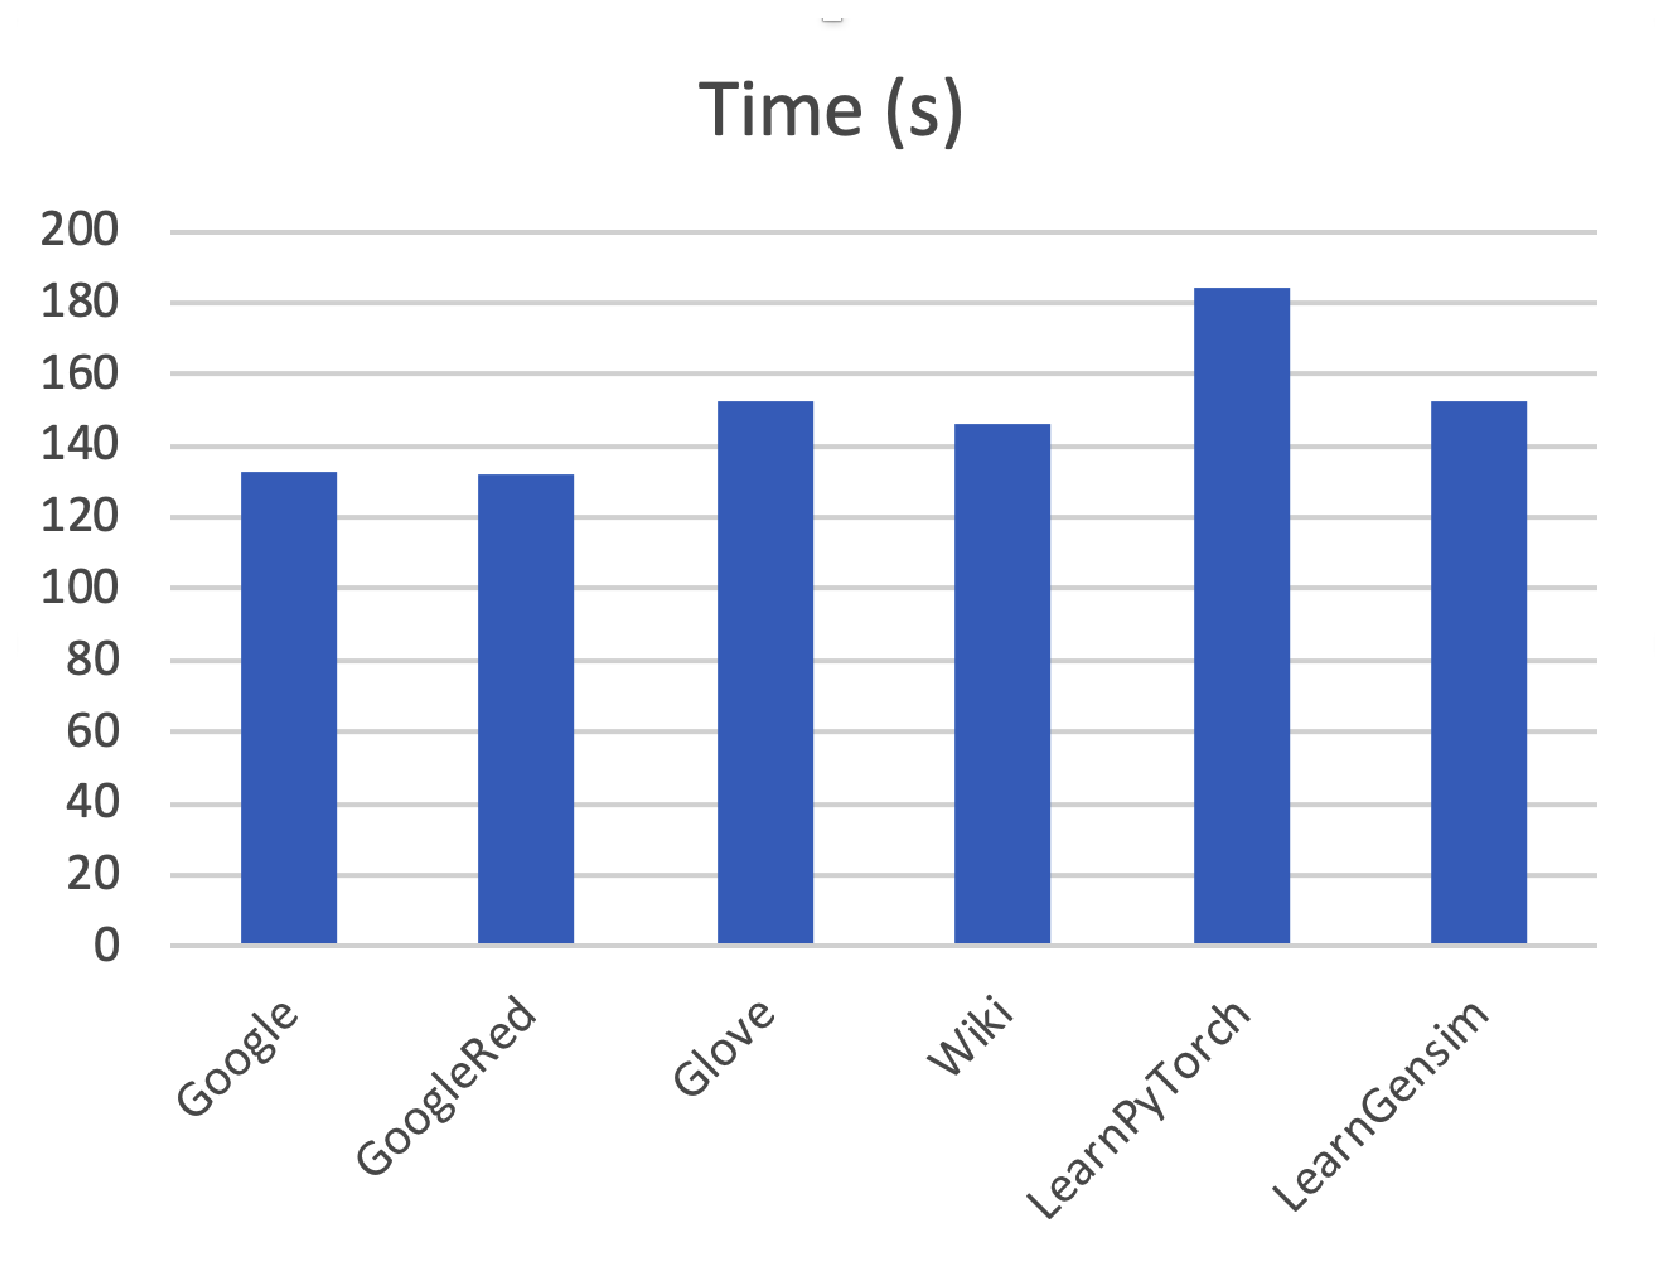
\includegraphics[width=0.5\textwidth]{time.eps}
    \caption{Time comparisons between models}
    \label{picture:time}
\end{figure}

Let's have a look at the main results of this paper: pictures \ref{picture:google}, \ref{picture:googlered}, \ref{picture:glove}, \ref{picture:wiki}, \ref{picture:learnpytorch} and \ref{picture:learngensim} show how the embedding model affect performances of the networks. MAP results are in blue, while MRR are in orange. After lot of tests, the results show clearly that the best embedding model is $GoogleRed$, that is, a version of $Google$ filtered to remove all words that are not contained in English dictionaries \cite{git}. Given the smaller dimension and the removal of junk-words, it shows faster execution times and better performances than any other embedding model. Moreover, given that this models have to be finally loaded in the GPU memory, it allows the usage of bigger batches, in particular when the GPU memory is not really large.

\begin{figure}[ht]
    \centering
    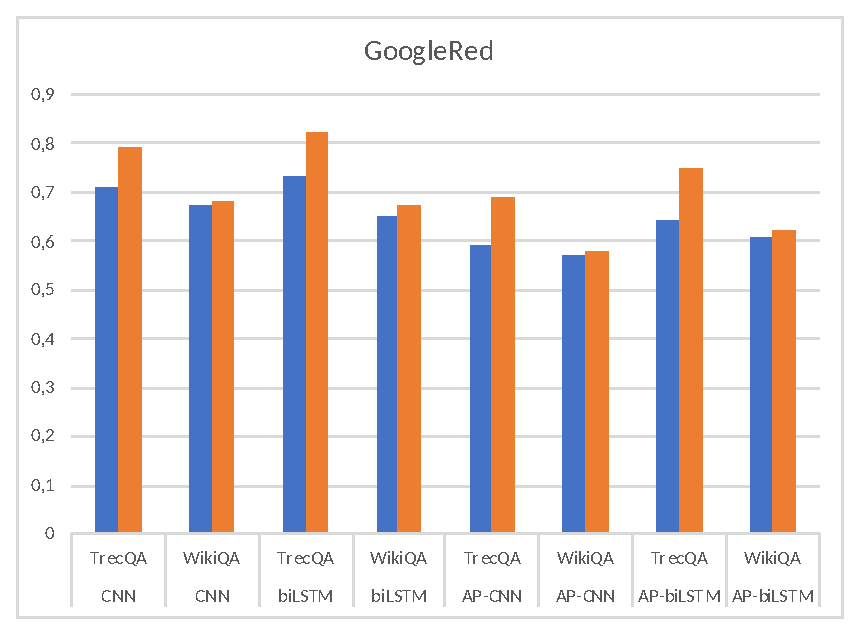
\includegraphics[width=0.5\textwidth]{google.eps}
    \caption{Performances of $GoogleRed$ embedding model}
    \label{picture:google}
\end{figure}
\begin{figure}[ht]
    \centering
    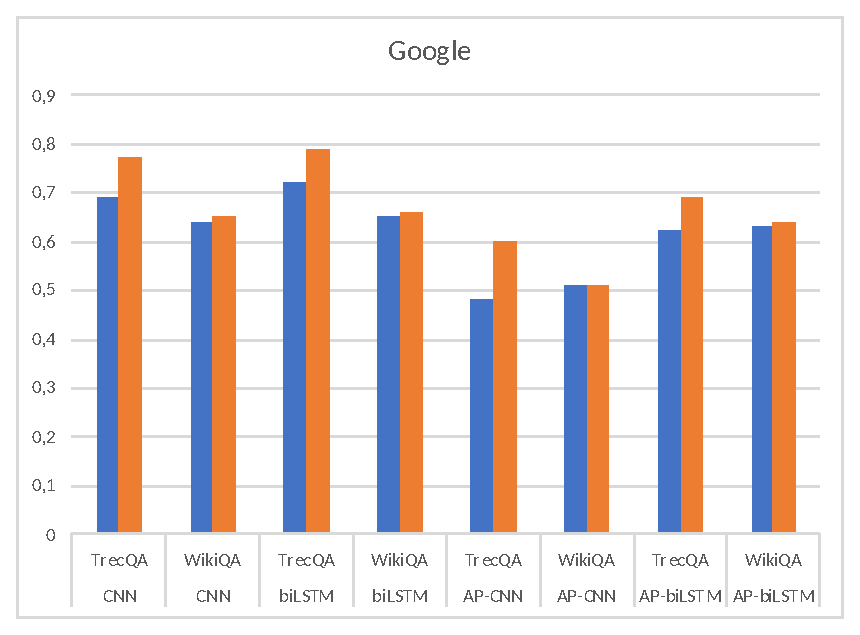
\includegraphics[width=0.5\textwidth]{googlered.eps}
    \caption{Performances of $Google$ embedding model}
    \label{picture:googlered}
\end{figure}
\begin{figure}[ht]
    \centering
    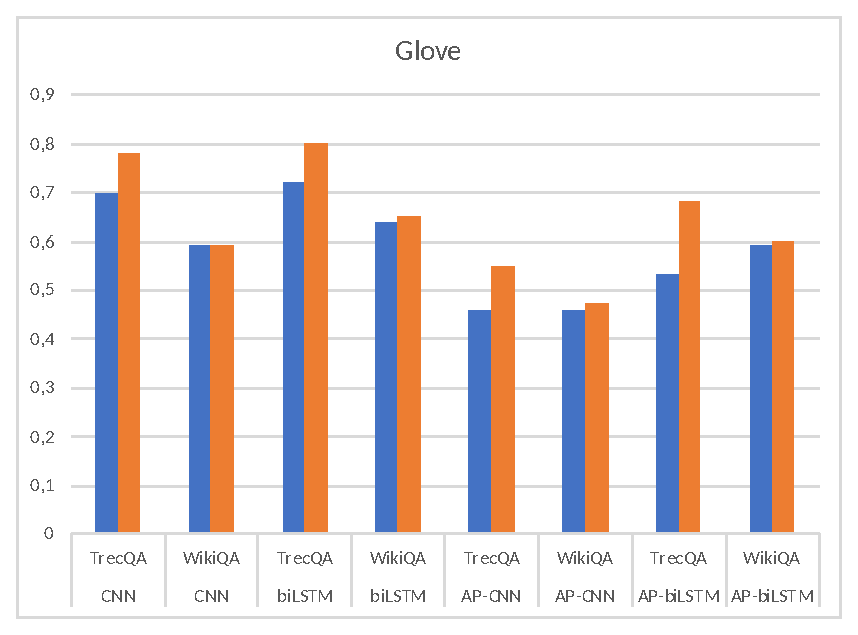
\includegraphics[width=0.5\textwidth]{glove.eps}
    \caption{Performances of $Glove$ embedding model}
    \label{picture:glove}
\end{figure}
\begin{figure}[ht]
    \centering
    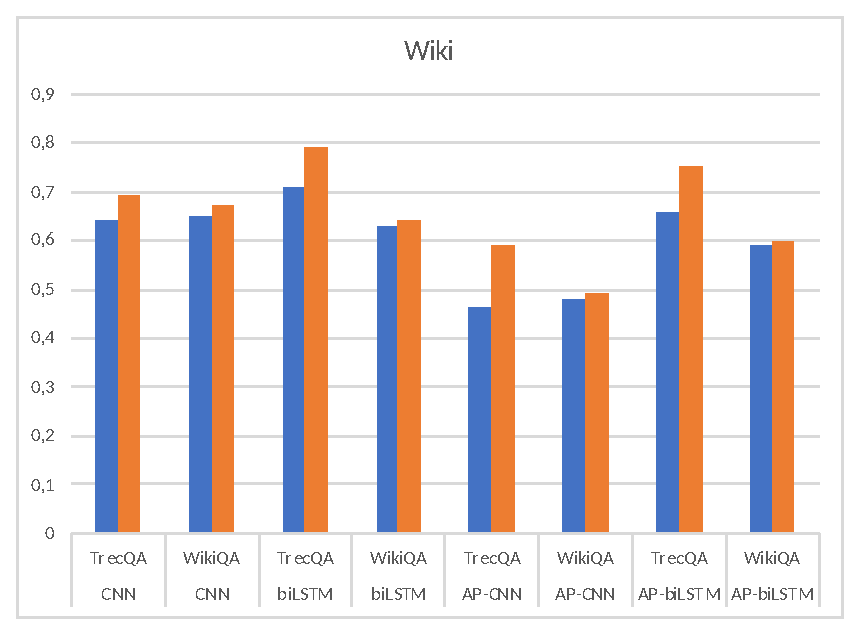
\includegraphics[width=0.5\textwidth]{wiki.eps}
    \caption{Performances of $Wiki$ embedding model}
    \label{picture:wiki}
\end{figure}
\begin{figure}[ht]
    \centering
    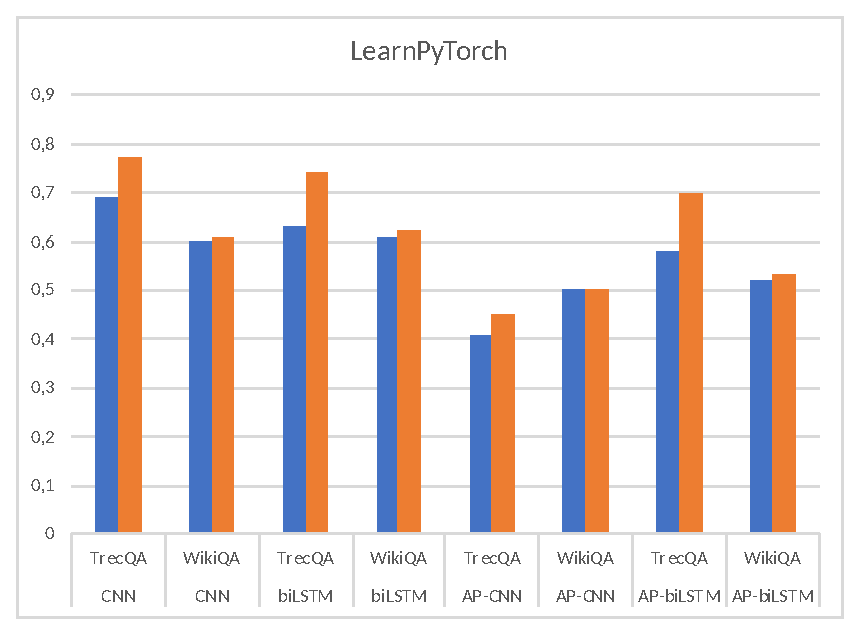
\includegraphics[width=0.5\textwidth]{learnpytorch.eps}
    \caption{Performances of $LearnPyTorch$ embedding model}
    \label{picture:learnpytorch}
\end{figure}
\begin{figure}[ht]
    \centering
    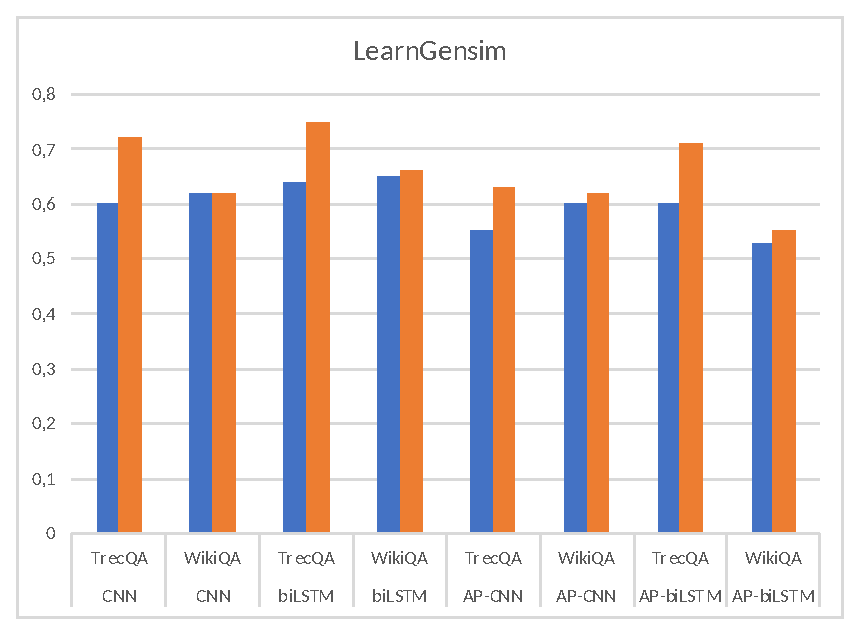
\includegraphics[width=0.5\textwidth]{learngensim.eps}
    \caption{Performances of $LearnGensim$ embedding model}
    \label{picture:learngensim}
\end{figure}

\clearpage

\bibliography{acl2018}
\bibliographystyle{plain}

\end{document}

